% Options for packages loaded elsewhere
\PassOptionsToPackage{unicode}{hyperref}
\PassOptionsToPackage{hyphens}{url}
%
\documentclass[
]{book}
\title{The Research Data Management Workbook}
\author{Kristin Briney}
\date{2023-09-26}

\usepackage{amsmath,amssymb}
\usepackage{lmodern}
\usepackage{iftex}
\ifPDFTeX
  \usepackage[T1]{fontenc}
  \usepackage[utf8]{inputenc}
  \usepackage{textcomp} % provide euro and other symbols
\else % if luatex or xetex
  \usepackage{unicode-math}
  \defaultfontfeatures{Scale=MatchLowercase}
  \defaultfontfeatures[\rmfamily]{Ligatures=TeX,Scale=1}
\fi
% Use upquote if available, for straight quotes in verbatim environments
\IfFileExists{upquote.sty}{\usepackage{upquote}}{}
\IfFileExists{microtype.sty}{% use microtype if available
  \usepackage[]{microtype}
  \UseMicrotypeSet[protrusion]{basicmath} % disable protrusion for tt fonts
}{}
\makeatletter
\@ifundefined{KOMAClassName}{% if non-KOMA class
  \IfFileExists{parskip.sty}{%
    \usepackage{parskip}
  }{% else
    \setlength{\parindent}{0pt}
    \setlength{\parskip}{6pt plus 2pt minus 1pt}}
}{% if KOMA class
  \KOMAoptions{parskip=half}}
\makeatother
\usepackage{xcolor}
\IfFileExists{xurl.sty}{\usepackage{xurl}}{} % add URL line breaks if available
\IfFileExists{bookmark.sty}{\usepackage{bookmark}}{\usepackage{hyperref}}
\hypersetup{
  pdftitle={The Research Data Management Workbook},
  pdfauthor={Kristin Briney},
  hidelinks,
  pdfcreator={LaTeX via pandoc}}
\urlstyle{same} % disable monospaced font for URLs
\usepackage{longtable,booktabs,array}
\usepackage{calc} % for calculating minipage widths
% Correct order of tables after \paragraph or \subparagraph
\usepackage{etoolbox}
\makeatletter
\patchcmd\longtable{\par}{\if@noskipsec\mbox{}\fi\par}{}{}
\makeatother
% Allow footnotes in longtable head/foot
\IfFileExists{footnotehyper.sty}{\usepackage{footnotehyper}}{\usepackage{footnote}}
\makesavenoteenv{longtable}
\usepackage{graphicx}
\makeatletter
\def\maxwidth{\ifdim\Gin@nat@width>\linewidth\linewidth\else\Gin@nat@width\fi}
\def\maxheight{\ifdim\Gin@nat@height>\textheight\textheight\else\Gin@nat@height\fi}
\makeatother
% Scale images if necessary, so that they will not overflow the page
% margins by default, and it is still possible to overwrite the defaults
% using explicit options in \includegraphics[width, height, ...]{}
\setkeys{Gin}{width=\maxwidth,height=\maxheight,keepaspectratio}
% Set default figure placement to htbp
\makeatletter
\def\fps@figure{htbp}
\makeatother
\setlength{\emergencystretch}{3em} % prevent overfull lines
\providecommand{\tightlist}{%
  \setlength{\itemsep}{0pt}\setlength{\parskip}{0pt}}
\setcounter{secnumdepth}{5}
\usepackage{booktabs}
\usepackage{graphicx}
\ifLuaTeX
  \usepackage{selnolig}  % disable illegal ligatures
\fi
\usepackage[]{natbib}
\bibliographystyle{plainnat}

\begin{document}
\maketitle


\includegraphics{./images/cover.jpg}

{
\setcounter{tocdepth}{1}
\tableofcontents
}
\hypertarget{about-this-book}{%
\chapter*{About this Book}\label{about-this-book}}
\addcontentsline{toc}{chapter}{About this Book}

\hypertarget{description}{%
\section*{Description}\label{description}}
\addcontentsline{toc}{section}{Description}

The Research Data Management Workbook is made up of a collection of exercises for researchers to improve their data management. The Workbook contains exercises across the data lifecycle, though the range of activities is not comprehensive. Instead, exercises focus on discrete practices within data management that are structured and can be reproduced by any researcher.

The book is divided into chapters, loosely by phases of the data lifecycle, with one or more exercises in each chapter. Every exercise comes with a description of its value within data management, instructions on how to do the exercise, original source of the exercise (when applicable), and the exercise itself.

The Workbook is intended as a supplement to existing data management education. If you would like to learn more about the principles of data management, please see the article ``Foundational Practices of Research Data Management'' \citep{briney_foundational_2020} or read the book ``Data Management for Researchers'' \citep{briney_data_2015}.

\hypertarget{edition}{%
\section*{Edition}\label{edition}}
\addcontentsline{toc}{section}{Edition}

This is edition 1.0 of The Research Data Management Workbook.

ISBN (PDF): 978-1-60049-015-6

ISBN (EPUB): 978-1-60049-014-9

I'm happy to receive any feedback on the Workbook to improve it for the next edition; you can message me at briney@caltech.edu.

\hypertarget{license}{%
\section*{License}\label{license}}
\addcontentsline{toc}{section}{License}

This book is available under a Creative Commons Attribution-NonCommercial (CC BY-NC) 4.0 International license.

I encourage you to use and adapt all of the exercises in this book for educational and personal use. Just remember to cite me:

\begin{itemize}
\tightlist
\item
  Briney, K. (2023). \emph{The Research Data Management Workbook.} Caltech Library. \url{https://doi.org/10.7907/z6czh-7zx60}
\end{itemize}

\hypertarget{the-author}{%
\section*{The Author}\label{the-author}}
\addcontentsline{toc}{section}{The Author}

\begin{figure}
\centering
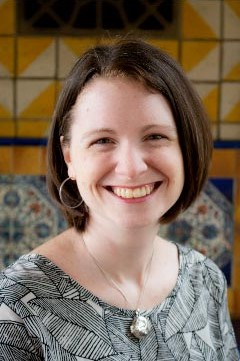
\includegraphics{images/00_KristinBriney.jpg}
\caption{Headshot of author, Kristin Briney. Image is of a smiling white woman with chin-length brown hair.}
\end{figure}

Kristin Briney is the Biology \& Biological Engineering Librarian at the California Institute of Technology and author of the books ``Data Management for Researchers'' \citep{briney_data_2015} and, with Becky Yoose, ``Managing Data for Patron Privacy'' \citep{briney_managing_2022}. She has a PhD in chemistry and an MLIS, both from the University of Wisconsin-Madison. Her research focuses on research data management, institutional data policy, and patron privacy vis-a-vis library data handling. Kristin is an advocate for the adoption of the international date standard ISO 8601 (YYYY-MM-DD) and likes to spend her free time making data visualizations out of yarn and fabric.

\hypertarget{introduction}{%
\chapter{Introduction}\label{introduction}}

\hypertarget{what-rdm}{%
\section{What is Research Data Management?}\label{what-rdm}}

Research data management is a set of collective practices and decisions that make it easier for you, your collaborators, and your future self to find, understand, and use your research data. These practices cover the entire lifecycle of research data, from its collection and analysis through sharing and reuse. There is no one magical data management practice to rule them all. Rather, data management consists of a number of small activities that make dealing with your data a better experience. Research is hard enough as it is without having to fight with your files, so the goal of data management is for you to maximize your time doing research instead of spending extra time with file handling.

\hypertarget{why-rdm}{%
\section{Why do Research Data Management?}\label{why-rdm}}

Most researchers have spent time, at some point in their careers, digging through their computer to find a specific file that can't be located. It's incredibly frustrating and a waste of time and resources, especially if you end up recollecting missing data. The good news is that it is possible to avoid this situation entirely by strategically managing your data better.

Done well, research data management means:

\begin{itemize}
\tightlist
\item
  always understanding what your data is and how you collected it even if the data is a year old
\item
  always finding the file you need quickly
\item
  never losing your data even if your hard drive crashes
\item
  knowing what rights and responsibilities you have over your data
\item
  knowing how and where to share your data to comply with your funder's data sharing policy
\item
  being able to pick up and easily reuse data from a past project
\end{itemize}

If all of those things sound like something you would like to implement in your research, you are reading the right book!

\hypertarget{how-rdm}{%
\section{How to Use this Book to Manage Your Research Data Better}\label{how-rdm}}

The Research Data Management Workbook is focused entirely on the ``how'' of data management. The Workbook consists of a series of worksheets, checklists, and procedures to set up new data management practices, check existing practices, and make good decisions about your data. You will find exercises covering all the ideals listed in the \protect\hyperlink{why-rdm}{``Why Do Research Data Management?'' section} above, allowing you to streamline your use of research data.

The Workbook is not a complete set of exercises for everything under the umbrella of data management. Instead, the Workbook centers on activities that are structured, reproducible, and apply to many researchers. The strength and weakness of data management is that many of its practices are customizable to individual research workflows. Each exercise in the Workbook, therefore, is built on best principles while allowing for customization to suit local needs.

You may go through exercises in the Workbook collectively or individually as you chose. Do note that some exercises require completing one or more other exercises in the book, so it's best to have the whole workbook on hand just in case. Finally, for the exercises that have been formatted as worksheets, I recommend printing them out and writing your answers in the space provided.

\hypertarget{more-rdm}{%
\section{Further Resources on Research Data Management}\label{more-rdm}}

``The Research Data Management Workbook'' does not comprehensively explain data management and therefore works best for those with some foundational data management knowledge or in tandem with other educational resources on research data management.

My best recommendation is to use the Workbook as the exercise book for my first book, ``Data Management for Researchers'' \citep{briney_data_2015}. The following table lays out how chapters in the Workbook match with chapters in ``Data Management for Researchers,'' allowing you to look up more information on any topic covered by the Workbook:

\begin{longtable}[]{@{}
  >{\raggedright\arraybackslash}p{(\columnwidth - 2\tabcolsep) * \real{0.33}}
  >{\raggedright\arraybackslash}p{(\columnwidth - 2\tabcolsep) * \real{0.29}}@{}}
\toprule
\begin{minipage}[b]{\linewidth}\raggedright
Research Data
Management Workbook
\end{minipage} & \begin{minipage}[b]{\linewidth}\raggedright
Data Management
for Researchers
\end{minipage} \\
\midrule
\endhead
Chapter 2 & Chapter 4 \\
Chapter 3 & Chapter 5 \\
Chapter 4 & Chapter 8 \\
Chapter 5 & Chapter 3 \\
Chapter 6 & Chapter 10 \\
Chapter 7 & Chapter 9 \\
\bottomrule
\end{longtable}

\hypertarget{documentation}{%
\chapter{Documentation}\label{documentation}}

Documentation has sometimes been called ``a love letter to your future self'' as it helps you remember important details about your research data. The great thing about research documentation is that it's not limited to a laboratory or research notebook, though notebooks are still very important! This chapter introduces two types of useful documentation -- a project-level README.txt and a data dictionary -- and offers worksheets for writing both. The chapter also includes a worksheet to evaluate an older entry in your laboratory notebook to ensure your documentation is of sufficient quality.

\hypertarget{lab-notebook}{%
\section{Evaluate a Laboratory Notebook}\label{lab-notebook}}

\textbf{\emph{Description:}} \emph{The laboratory or research notebook is a fundamental documentation method for many researchers. But for how ubiquitous the lab notebook is, documentation can sometimes be lacking. The ideal laboratory notebook allows someone with similar training as you to be able to follow everything you did in your research. This exercise prompts you to review an old entry within your laboratory notebook to evaluate if your documentation is sufficient for reproducing your work.}

\textbf{\emph{Instructions:}} \emph{You will need a laboratory notebook entry from 6-12 months ago to do this exercise. Once you have the entry, read through it to try to understand what you did on that day. Answer the exercise questions to evaluate the entry and identify any note keeping improvements to make.}

\begin{center}\rule{0.5\linewidth}{0.5pt}\end{center}

\textbf{Date of lab notebook entry being evaluated:} \_\_\_\_\_\_\_\_\_\_\_\_\_\_\_\_\_\_\_\_

\textbf{Read the entry and summarize the work you did on that date:}

~

~

~

\textbf{How easy was it to understand the work you did from your notes?}

~

~

~

\textbf{Could you reproduce your work based on the information in your notes? If not, what extra information do you need?}

~

~

~

\textbf{What worked well with your note keeping?}

~

~

~

\textbf{What should you improve about your note keeping?}

~

~

~

\textbf{List one change you will implement to take better research notes:}

~

~

~

\hypertarget{readme-txt}{%
\section{Write a Project-Level README.txt}\label{readme-txt}}

\textbf{\emph{Description:}} \emph{Data files living on a computer often need extra documentation for someone to understand what research they correspond to. In particular, it is useful to record the most basic project information and store it in the top-level folder of each research project. This can be done with a README.txt. The name, ``README'', indicates that the file conveys important information and the file type, TXT, can be opened by many different software programs, making the content maximally accessible. This exercise walks you through the key information needed in a project-level README.txt file. The same information can also be recorded at the front of a physical laboratory notebook.}

\textbf{\emph{Instructions:}} \emph{Pick a research project and answer the following questions. Copy all of the text into a TXT file and save it with the name ``README.txt''. Store this file in the top-level of the project folder on your computer, alongside the project files.}

\textbf{\emph{Source:}} \emph{This exercise was adapted from the ``Project Close Out Checklist'' \citep{briney_project_2020}.}

\begin{center}\rule{0.5\linewidth}{0.5pt}\end{center}

\textbf{Project documented by this README.txt:} \_\_\_\_\_\_\_\_\_\_\_\_\_\_\_\_\_\_\_\_

\textbf{Write a brief project description:}

\emph{Example: The Data Doubles project was a 4-year, IMLS-funded research project examining student perceptions of privacy in library learning analytics.}

~

~

~

\textbf{What is the time period the project was done over?}

\emph{Example: The project was conducted between summer 2018 and summer 2022.}

~

~

~

\textbf{Who worked on the project?}

\emph{Example: Eight researchers from eight different instutions worked on the project, including: KMLJ, AA, KB, AG, MP, MR, DS, and MS.}

~

~

~

\textbf{Where are the data, code, and other files are stored?}

\emph{Example: Research files are stored on Google Drive, with the exception that participant data is stored in IU-hosted Box. Survey data is also in Qualtrics. Code is on GitHub. The shared literature library is in Zotero.}

~

~

~

\textbf{How and where is the project documented?}

\emph{Example: Documentation for the project is in Google Drive. Notes on team decisions from meetings are in the DataDoubles/Meetings folder. Notes on data are in the DataDoubles/Research folder.}

~

~

~

\textbf{How are files organized? Are any naming conventions used and, if so, what are they (see \protect\hyperlink{file-organization-and-naming}{Chapter 3})?}

\emph{Example: All data is in the DataDoubles/Data folder, with subfolders labelled by interview theme code. Each site has its own folder within the project folder for individual site files. Interview data files are named with: interview theme, site, interview ID, interview date, and data type/analysis stage (e.g.~``PRO\_BL03\_20180222\_Audio.mp3'' and ``AWA\_MK01\_20180222\_Notes.pdf''). Please see the living data management plan for complete set of codes and more details.}

~

~

~

\textbf{What else does someone need to know to understand these files?}

\emph{Example: Additional documentation on the project and public research files are available on OSF.}

~

~

~

\hypertarget{data-dictionary}{%
\section{Create a Data Dictionary}\label{data-dictionary}}

\textbf{\emph{Description:}} \emph{Ideally, a spreadsheet is formatted with a row of variable names at the top, followed by rows of data going down. This makes easy for data to be used in any data analysis software (interoperability is a good thing) but makes it impossible to document a spreadsheet within the file itself. For this reason, it's useful to create a data dictionary to describe the spreadsheet so that others can interpret the data. This exercise walks you through the major information you should record for each variable in the spreadsheet, adding up to a complete dictionary to accompany the spreadsheet file.}

\textbf{\emph{Instructions:}} \emph{Pick one spreadsheet variable and record its information in the corresponding rows of the table. Repeat this process for the remaining variables in the spreadsheet. Copy all information into a text document and save it next to the spreadsheet. It is useful to save the data dictionary with the same root name as its data file by appending ``\_dictionary'' on the end of the file name; for example, the data dictionary for the file ``myData.xlsx'' would be ``myData\_dictionary.txt''.}

\textbf{\emph{Source:}} \emph{This exercise was adapted from ``Leveling Up Data Management'' \citep{briney_leveling_2023}.}

\begin{center}\rule{0.5\linewidth}{0.5pt}\end{center}

\begin{longtable}[]{@{}
  >{\raggedright\arraybackslash}p{(\columnwidth - 2\tabcolsep) * \real{0.33}}
  >{\raggedright\arraybackslash}p{(\columnwidth - 2\tabcolsep) * \real{0.60}}@{}}
\toprule
\begin{minipage}[b]{\linewidth}\raggedright
Question
\end{minipage} & \begin{minipage}[b]{\linewidth}\raggedright
Example
\end{minipage} \\
\midrule
\endhead
Variable name & \emph{site} \\
Variable description & \emph{Two-letter abbreviation describing the
name of the overall site where the sample
was collected.} \\
Variable units & \emph{N/A} \\
Relationship to
other variables & \emph{Partner to variable ``sampleNum'', which
together define the sample ID (site name +
sample number at that site). Related to
variables ``latitude'' and ``longitude'',
which record exact coordinate location
and are more specific than the larger
site code.} \\
Variable coding
values and meanings & \emph{Coding values and meanings:
BL = Badlands NP;
DV = Death Valley NP;
GT = Grand Teton NP;
JT = Joshua Tree NP;
ZN = Zion NP} \\
Known issues with
the data & \emph{Some Badlands samples were collected
outsideof the park boundaries; see latitude
and longitude variables for specific
locations.} \\
Anything else to
know about the data? & \emph{Older data (pre-2013) used one-letter
abbreviations for site code but this was
updated for clarity and ease of
identification.} \\
\bottomrule
\end{longtable}

~

\begin{longtable}[]{@{}
  >{\raggedright\arraybackslash}p{(\columnwidth - 2\tabcolsep) * \real{0.33}}
  >{\raggedright\arraybackslash}p{(\columnwidth - 2\tabcolsep) * \real{0.60}}@{}}
\toprule
\begin{minipage}[b]{\linewidth}\raggedright
Question
\end{minipage} & \begin{minipage}[b]{\linewidth}\raggedright
Variable
\end{minipage} \\
\midrule
\endhead
Variable name
~~~
~~~
~~~
~~~
~~~
~~~
~~~
~~~
~~~
~~~
~~~
~~~
~~~
~~~
~~~
~~~
~~~
~~~
~~~
~~~
~~~
~~~
~~~
~~~
~~~
~~~ & ~ \\
Variable description
~~~
~~~
~~~
~~~
~~~
~~~
~~~
~~~
~~~
~~~
~~~
~~~
~~~
~~~
~~~
~~~
~~~
~~~
~~~
~~~
~~~
~~~
~~~
~~~ & ~ \\
Variable units
~~~
~~~
~~~
~~~
~~~
~~~
~~~
~~~
~~~
~~~
~~~
~~~
~~~
~~~
~~~
~~~
~~~
~~~
~~~
~~~
~~~
~~~
~~~
~~~
~~~
~~~ & ~ \\
Relationship to
other variables
~~~
~~~
~~~
~~~
~~~
~~~
~~~
~~~
~~~
~~~
~~~ & ~ \\
Variable coding
values and meanings
~~~
~~~
~~~
~~~
~~~
~~~
~~~
~~~
~~~
~~~
~~~ & ~ \\
Known issues with
the data
~~~
~~~
~~~
~~~
~~~
~~~
~~~
~~~
~~~
~~~
~~~
~~~
~~~
~~~ & ~ \\
Anything else to
know about the data?
~~~
~~~
~~~
~~~
~~~
~~~
~~~
~~~
~~~
~~~
~~~ & ~ \\
\bottomrule
\end{longtable}

\hypertarget{file-organization-and-naming}{%
\chapter{File Organization and Naming}\label{file-organization-and-naming}}

Good file organization and naming are foundational data management practices, as they help you find files quickly when you need them. To set up file organization and naming conventions, this chapter offers two exercises: a card-sorting process for brainstorming a file organization system; and a worksheet for creating a file naming convention for a group of files.

\hypertarget{file-organization}{%
\section{Set Up a File Organization System}\label{file-organization}}

\textbf{\emph{Description:}} \emph{Implementing a file organization system is the first step toward creating order for your research data. Well-organized files make it easier to find the data you need without spending lots of time searching your computer. Every researcher organizes their files slightly differently, but the actual organizational system is less important that having a place where all of your files should logically go. This exercise prompts you to brainstorm organizational groupings and hierarchies to come up with an order for managing your research data.}

\textbf{\emph{Instructions:}} \emph{This is a card-sorting exercise, meaning you will need a stack of note cards or post-it notes to do this activity, ideally in three different colors. Follow the instructions to label cards and move them around until you develop your organizational system. There is no one correct way to do this so feel free to play around, add new cards, and move cards however you want! Once you put your new organizational system into place, be sure to always put your files where they're supposed to go.}

\begin{figure}
\centering
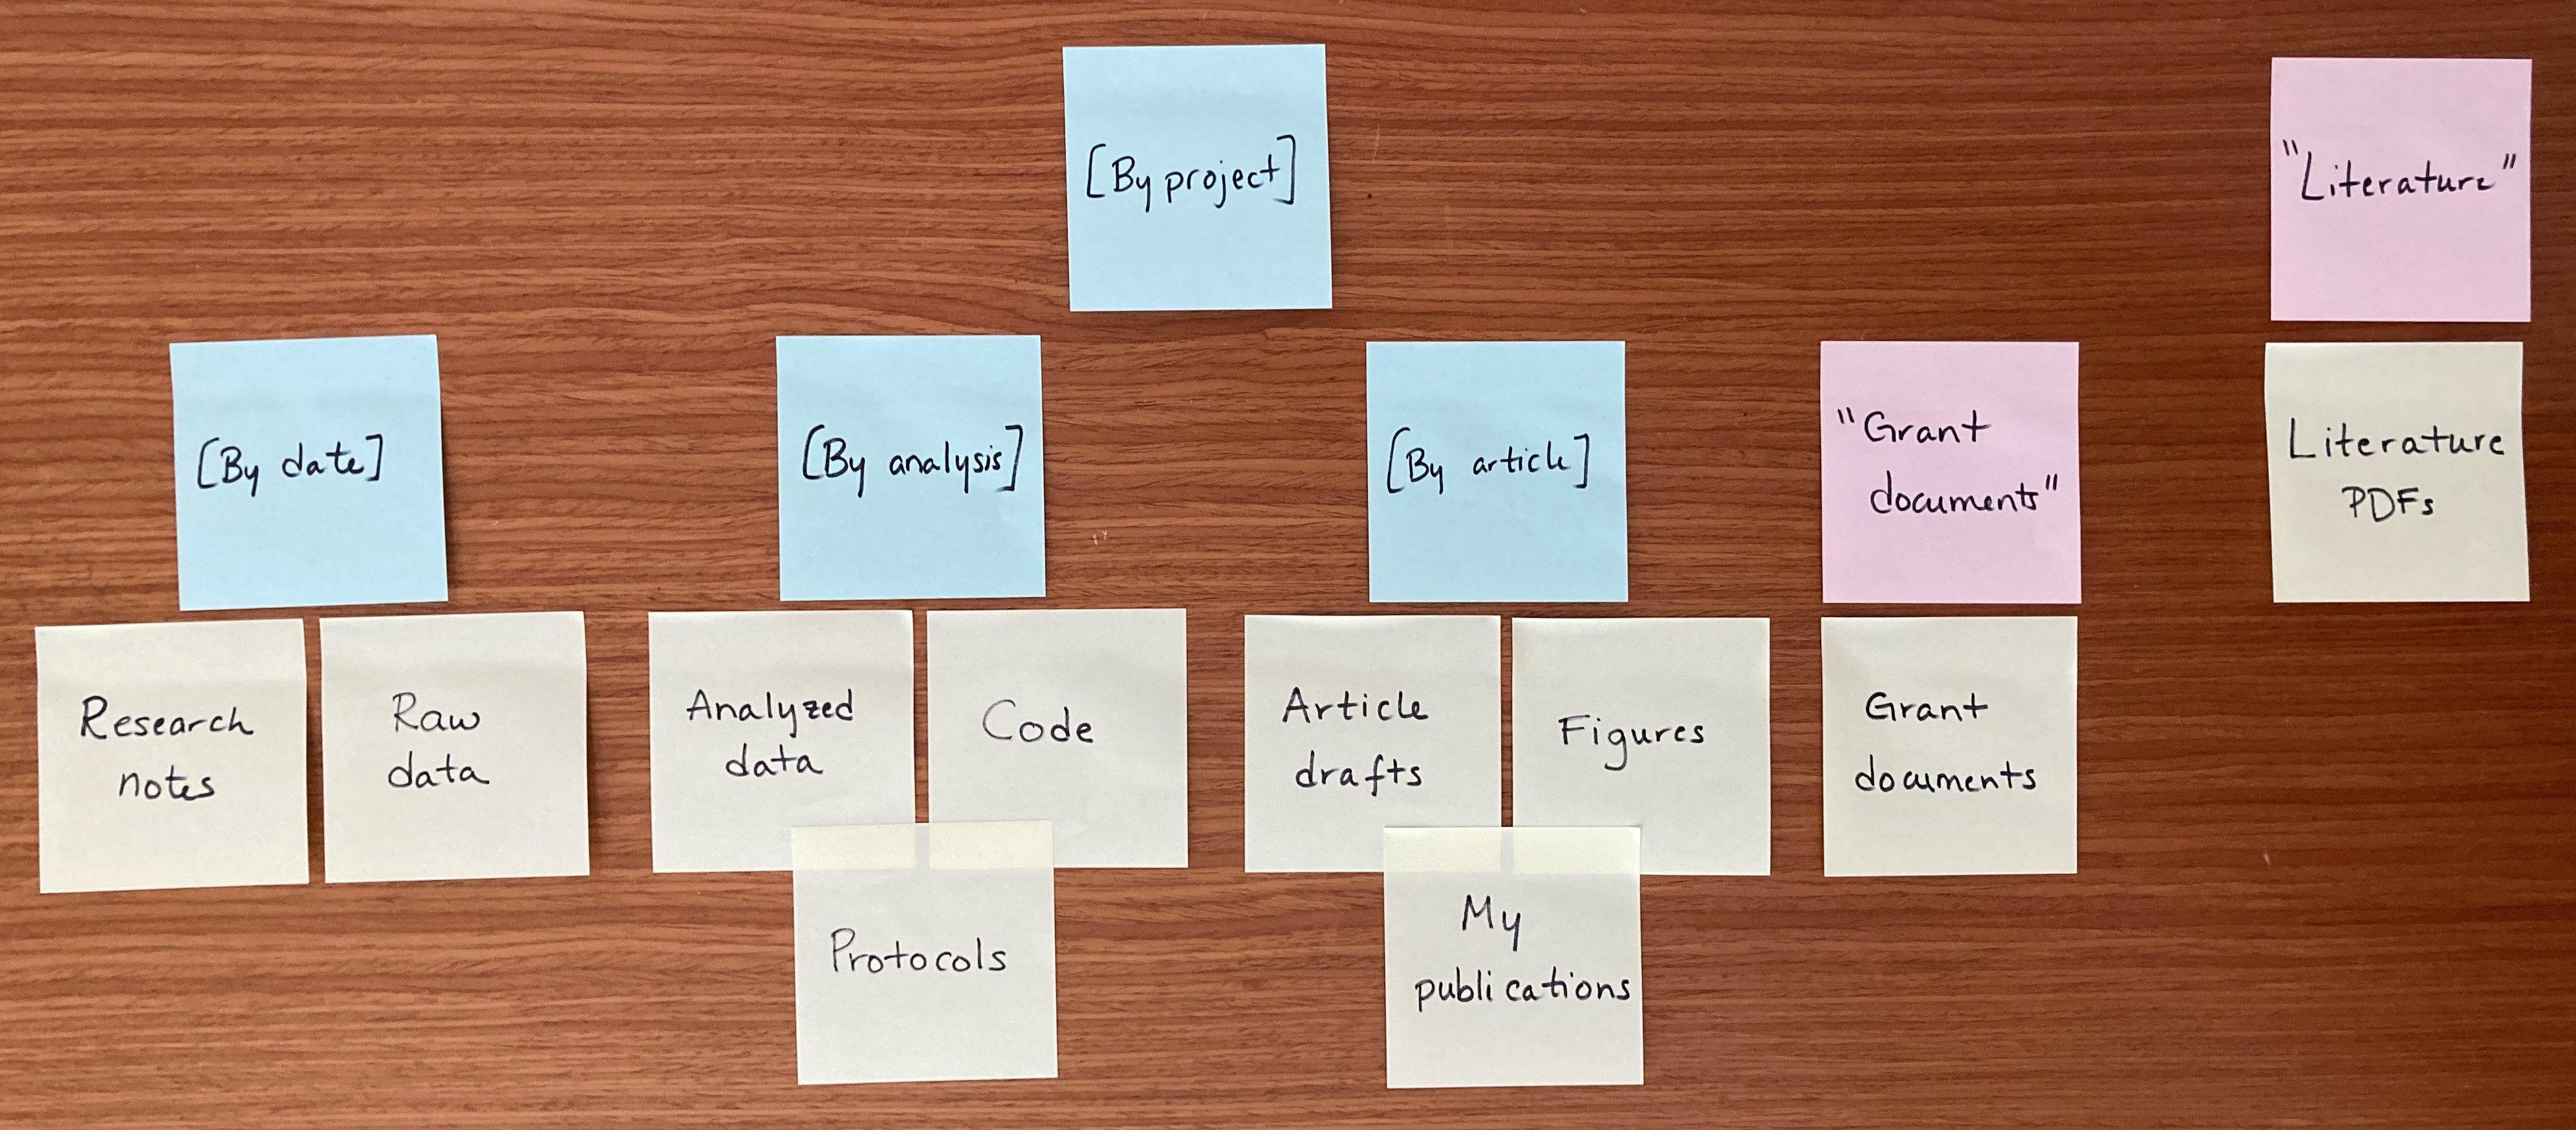
\includegraphics{images/03_CardSorting.jpg}
\caption{Example of organizational exercise. Image is of blue (group folder), pink (single folder), and yellow (data type) sticky notes, each with its own label, organized hierarchically on a wooden desktop.}
\end{figure}

\begin{center}\rule{0.5\linewidth}{0.5pt}\end{center}

\begin{enumerate}
\def\labelenumi{\arabic{enumi}.}
\tightlist
\item
  Take a stack of note cards or post-it notes in the first color and write the following labels on one card each, omitting any file types that you do not use in your research:

  \begin{itemize}
  \tightlist
  \item
    Raw data
  \item
    Analyzed data
  \item
    Code
  \item
    Protocols
  \item
    Article drafts
  \item
    Figures
  \item
    My publications
  \item
    Literature PDFs
  \item
    Grant documents
  \item
    Research notes
  \end{itemize}
\item
  Move cards around and group together file-type cards that you want to store together. Files that will be stored near each other in a folder hierarchy, but not together, should be placed near each other while file types expected to be stored completely separately should be away from other cards.
\item
  Create hierarchies in file organization by adding new ``folder'' cards in one of two types; use different colored cards for each folder type:

  \begin{itemize}
  \tightlist
  \item
    Cards in the second color represent a single folder. These should be labeled with the folder name in quotations (e.g.~``Literature'' or ``My publications'').
  \item
    Cards in the third color represent a group of folders, such as for folders organized by date or by project. Use only one card to represent the organizational pattern that will be repeated. These cards should be labeled with the organizational system in square brackets (e.g.~{[}By date{]} or {[}By project{]}). Note: folders organized by date should, in real life, be labelled using the convention YYYYMMDD or YYYY-MM-DD to facilitate chronological sorting.
  \end{itemize}
\item
  Move existing file-type cards/groups of file-type cards underneath the new folder cards to show the hierarchy of how a file type will be saved in a specific folder or group of folders. Organizational-group folders (cards in the third color) only need to be represented once in the card sorting, as they are assumed to represent multiple folders on a computer.
\item
  Make copies of any type of card and add folder levels, as needed. Adjust placement and hierarchies until you are happy with the organizational system you developed.
\item
  Record your organizational system in your lab notebook and/or a \protect\hyperlink{readme-txt}{README.txt}.
\end{enumerate}

\hypertarget{file-naming}{%
\section{Create a File Naming Convention}\label{file-naming}}

\textbf{\emph{Description:}} \emph{File naming conventions are a simple way to add order to your files and help to find them later. Rich and descriptive file names make it easier to search for files, understand at a glance what they contain, and tell related files apart. This exercise guides researchers through the process of creating a file naming convention for a group of related files.}

\textbf{\emph{Instructions:}} \emph{Fill in each section for a group of related files following the instructions; an example for microscopy files is provided. This exercise may be redone as needed, as different groups of files require different naming conventions.}

\textbf{\emph{Source:}} \emph{This exercise is based on the ``File Naming Convention Worksheet'' \citep{briney_file_2020}.}

\begin{figure}
\centering
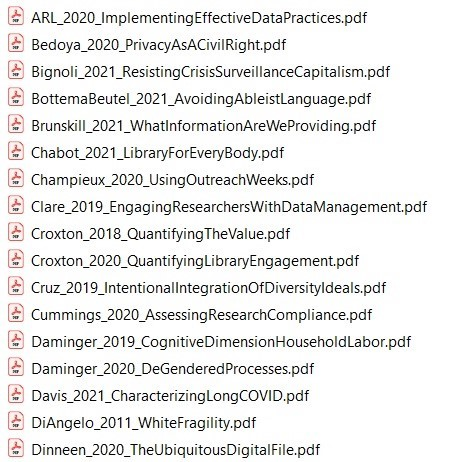
\includegraphics{images/03_FileNaming.jpg}
\caption{Screenshot of article pdf's in a file system with consistent file names. File names use the convention FirstAuthorLastName\_YEAR\_ShortTitle.pdf}
\end{figure}

\begin{center}\rule{0.5\linewidth}{0.5pt}\end{center}

\textbf{1. What group of files will this naming convention cover?}

You can use different conventions for different file sets.

\emph{Example: This convention will apply to all of my microscopy files, from raw image through processed image.}

~

~

~

\textbf{2. What information (metadata) is important about these files and makes each file distinct?}

Ideally, pick three pieces of metadata; use no more than five. This metadata should be enough for you to visually scan the file names and easily understand what's in each one.

\emph{Example: For my images, I want to know date, sample ID, and image number for that sample on that date.}

\begin{enumerate}
\def\labelenumi{\arabic{enumi}.}
\tightlist
\item
\item
\item
\item
\item
\end{enumerate}

\textbf{3. Do you need to abbreviate any of the metadata or encode it?}

If any of the metadata from step 2 is described by lots of text, decide what shortened information to keep. If any of the metadata from step 2 has regular categories, standardize the categories and/or replace them with 2- or 3-letter codes; be sure to document these codes.

\emph{Example: Sample ID will use a code made up of: a 2-letter project abbreviation (project 1 = P1, project 2 = P2); a 3-letter species abbreviation (mouse = ``MUS'', fruit fly = ``DRS''); and 3-digit sample ID (assigned in my notebook).}

~

~

~

\textbf{4. What is the order for the metadata in the file name?}

Think about how you want to sort and search for your files to decide what metadata should appear at the beginning of the file name. If date is important, use ISO 8601-formatted dates (YYYYMMDD or YYYY-MM-DD) at the beginning of the file names so dates sort chronologically.

\emph{Example: My sample ID is most important so I will list it first, followed by date, then image number.}

\begin{enumerate}
\def\labelenumi{\arabic{enumi}.}
\tightlist
\item
\item
\item
\item
\item
\end{enumerate}

\textbf{5. What characters will you use to separate each piece of metadata in the file name?}

Many computer systems cannot handle spaces in file names. To make file names both computer- and human-readable, use dashes (-), underscores (\_), and/or capitalize the first letter of each word in the file names. A good convention is to use underscores to separate unrelated pieces of metadata and dashes to separate related pieces of metadata for parsing and readability.

\emph{Example: I will use underscores to separate metadata and dashes between parts of my sample ID.}

~

~

~

\textbf{6. Will you need to track different versions of each file?}

You can track versions of a file by appending version information to end of the file name. Consider using a version number (e.g.~``v01'') or the version date (use ISO 8601 format: YYYYMMDD or YYYY-MM-DD).

\emph{Example: As each image goes through my analysis workflow, I will append the version type to the end of the file name (e.g.~``\_raw'', ``\_processed'', and ``\_composite'').}

~

~

~

\textbf{7. Write down your naming convention pattern.}

Make sure the convention only uses alphanumeric characters, dashes, and underscores. Ideally, file names will be 32 characters or less.

\emph{Example: My file naming convention is ``SA-MPL-EID\_YYYYMMDD\_\#\#\#\_status.tif'' Examples are ``P1-MUS-023\_20200229\_051\_raw.tif'' and ``P2-DRS-285\_20191031\_062\_composite.tif''.}

~

~

~

\textbf{8. Document this convention in a README.txt (or save this worksheet) and keep it with your files.}

~

~

~

\hypertarget{data-storage}{%
\chapter{Data Storage}\label{data-storage}}

All research data needs to be stored and backed up, but it can be frustrating to pick these systems and ensure that they are working correctly. This chapter consists of two exercises: a worksheet to document available storage and backup options and decide between them; and a procedure for testing that a backup system is working.

\hypertarget{storage}{%
\section{Pick Storage and Backup Systems}\label{storage}}

\textbf{\emph{Description:}} \emph{Research data needs to be stored and backed up reliably so that important data is not lost. But storage is commonly a challenge, as institutions don't always offer uniform options for storage and backup. This exercise prompts you to examine the storage and backup systems available to you before determining which is the best set of options for your data.}

\textbf{\emph{Instructions:}} \emph{Answer the questions and then fill out the table of information about each possible storage and backup systems. Examine all of the options, evaluating them based on the criteria listed below. Then select primary storage and backup systems and, optionally, an alternate backup.}

\begin{center}\rule{0.5\linewidth}{0.5pt}\end{center}

\textbf{What is the estimated total data storage you will need over the next five years?}

\emph{Example: I estimate that I will generate 100 GB of data over the next five years of my project.}

~

~

~

\textbf{Does your data require meeting any specific security standards? If so, what level of security?}

\emph{Example: My data will include some human subjects data, so my storage systems must have restrictions on access but it's not medical data so they don't have to be HIPAA compliant.}

~

~

~

\textbf{What storage and backup systems are available to you, such as through your institution, workplace, or elsewhere?}

\emph{Example: I have the following systems available to me: my computer, a Time Machine backup, a departmental server, institution-licensed Box account, and Google Drive.}

~

~

~

\textbf{Fill out the information in the table for \emph{each} storage and backup system you are considering:}

\begin{longtable}[]{@{}
  >{\raggedright\arraybackslash}p{(\columnwidth - 2\tabcolsep) * \real{0.33}}
  >{\raggedright\arraybackslash}p{(\columnwidth - 2\tabcolsep) * \real{0.60}}@{}}
\toprule
\begin{minipage}[b]{\linewidth}\raggedright
Question
\end{minipage} & \begin{minipage}[b]{\linewidth}\raggedright
Example
\end{minipage} \\
\midrule
\endhead
System name & \emph{Departmental server} \\
Is it storage or
backup? & \emph{Storage} \\
What is the cost? & \emph{No cost for 10GB and under.
Cost is \$5 per 10 GB per year after that.} \\
What is the hardware
type? & \emph{Server, exact hardware type unknown.} \\
Is the system
backed up? & \emph{No backup.} \\
For backup systems,
is backup automatic? & \emph{N/A} \\
What level of
security does the
system provide? & \emph{Storage is password protected.} \\
Is the system local
or remote? & \emph{System is local.} \\
Is there a limit
to storage capacity? & \emph{Storage limit is 500GB per research
group.} \\
Who manages the
system? & \emph{Departmental IT manages the server.} \\
Is it easy or
difficult to use? & \emph{Very easy to use once set up.} \\
\bottomrule
\end{longtable}

~

\begin{longtable}[]{@{}
  >{\raggedright\arraybackslash}p{(\columnwidth - 2\tabcolsep) * \real{0.33}}
  >{\raggedright\arraybackslash}p{(\columnwidth - 2\tabcolsep) * \real{0.60}}@{}}
\toprule
\begin{minipage}[b]{\linewidth}\raggedright
Question
\end{minipage} & \begin{minipage}[b]{\linewidth}\raggedright
System
\end{minipage} \\
\midrule
\endhead
System name
~~~
~~~
~~~
~~~
~~~
~~~
~~~
~~~
~~~
~~~
~~~
~~~
~~~
~~~
~~~
~~~
~~~
~~~
~~~
~~~
~~~
~~~
~~~
~~~
~~~
~~~ & ~ \\
Is it storage or
backup?
~~~
~~~
~~~
~~~
~~~
~~~
~~~
~~~
~~~
~~~
~~~
~~~
~~~
~~~
~~~
~~~
~~~
~~~
~~~
~~~
~~~
~~~ & ~ \\
What is the cost?
~~~
~~~
~~~
~~~
~~~
~~~
~~~
~~~
~~~
~~~
~~~
~~~
~~~
~~~
~~~
~~~
~~~
~~~
~~~
~~~
~~~
~~~
~~~
~~~ & ~ \\
What is the hardware
type?
~~~
~~~
~~~
~~~
~~~
~~~
~~~
~~~
~~~
~~~
~~~
~~~
~~~
~~~ & ~ \\
Is the system
backed up?
~~~
~~~
~~~
~~~
~~~
~~~
~~~
~~~
~~~
~~~
~~~
~~~
~~~
~~~ & ~ \\
For backup systems,
is backup automatic?
~~~
~~~
~~~
~~~
~~~
~~~
~~~
~~~
~~~
~~~
~~~
~~~
~~~
~~~ & ~ \\
What level of
security does the
system provide?
~~~
~~~
~~~
~~~
~~~
~~~
~~~
~~~
~~~
~~~
~~~
~~~
~~~
~~~ & ~ \\
Is the system local
or remote?
~~~
~~~
~~~
~~~
~~~
~~~
~~~
~~~
~~~
~~~
~~~
~~~
~~~
~~~ & ~ \\
Is there a limit
to storage capacity?
~~~
~~~
~~~
~~~
~~~
~~~
~~~
~~~
~~~
~~~
~~~ & ~ \\
Who manages the
system?
~~~
~~~
~~~
~~~
~~~
~~~
~~~
~~~
~~~
~~~
~~~
~~~
~~~
~~~ & ~ \\
Is it easy or
difficult to use?
~~~
~~~
~~~
~~~
~~~
~~~
~~~
~~~
~~~
~~~
~~~
~~~
~~~
~~~ & ~ \\
\bottomrule
\end{longtable}

\textbf{Optimize your storage and backups on the following considerations:}

\begin{enumerate}
\def\labelenumi{\arabic{enumi}.}
\tightlist
\item
  You need a primary storage system that:

  \begin{itemize}
  \tightlist
  \item
    will hold all of your data files,
  \item
    meets your needed level of security.
  \end{itemize}
\item
  You need one backup that:

  \begin{itemize}
  \tightlist
  \item
    will hold all of your data files,
  \item
    meets your needed level of security,
  \item
    is reliable/managed by someone you trust,
  \item
    is easy to use,
  \item
    backs up automatically.
  \end{itemize}
\item
  At least one backup should be in a different location than your main storage system for disaster resiliency. If your main backup is nearby your primary storage and/or if your primary storage system is not reliable, you need a second backup that:

  \begin{itemize}
  \tightlist
  \item
    will hold all of your files,
  \item
    meets your needed level of security,
  \item
    is reliable/managed by someone you trust.
  \end{itemize}
\end{enumerate}

\textbf{Pick your storage and backup systems:}

\emph{Example: My primary storage will be my computer with added security restrictions. I will use Time Machine as my first automatic backup and institutional Box, which is controlled access, as my second backup because it is remote.}

~

~

~

\hypertarget{backup}{%
\section{Test Your Backup}\label{backup}}

\textbf{\emph{Description:}} \emph{Backups are super important for your data, so it's always good to test that your backups are still working. Nothing is worse than losing your data from your primary storage and then realizing that your backup isn't working either. Beyond checking that your backup is working, it's also good to know how to recover your files so that you don't have to learn this for the first time while panicking about lost data. This short exercise walks you through getting a file off your backup to test that it is working and to learn how the data-recovery process works.}

\textbf{\emph{Instructions:}} \emph{Pick a backup system and a file to recover and work through the steps. The hard part of this exercise is finding instructions for file recovery and recovering the file, which vary by backup system.}

\begin{center}\rule{0.5\linewidth}{0.5pt}\end{center}

\begin{enumerate}
\def\labelenumi{\arabic{enumi}.}
\tightlist
\item
  Identify where your data is backed up.
\item
  Find instructions for recovering data from your backup system.
\item
  Pick a data file from your computer.
\item
  Follow the instructions from step 2 to get a copy of the data file from step 3 out of your backup system.
\item
  If this process didn't work, fix your backup system. If this process did work, congrats your backup is working and you know how to recover your files!
\end{enumerate}

\hypertarget{data-management}{%
\chapter{Data Management}\label{data-management}}

While this entire workbook covers data management activities, it's often useful to take a step back and document the data management decisions that have been made. This chapter provides exercises in documenting data management in two areas: a worksheet for writing a living data management plan (which builds on exercises from previous chapters); and a worksheet for discussing roles and responsibilities around data management with your research collaborators.

\hypertarget{living-dmp}{%
\section{Write a Living Data Management Plan (DMP)}\label{living-dmp}}

\textbf{\emph{Description:}} \emph{Many researchers are aware of the two-page data management plan (DMP) for a grant application, but you may not be aware of the more useful type of DMP: a living DMP. This document describes how data will be actively managed during a project and may be updated whenever necessary to reflect current data practices. A living DMP is a useful touchstone for understanding where data lives, how it's labelled, how it moves through the research process, and who will oversee the data management. This exercise guides you through the process of creating a living DMP for your research.}

\textbf{\emph{Instructions:}} \emph{Pick a project and answer the following questions to build your living DMP. This DMP may be changed at any time to improve practices. If you are doing collaborative research, work through this exercise with your collaborators to agree on shared conventions.}

\begin{center}\rule{0.5\linewidth}{0.5pt}\end{center}

\textbf{Write a short summary of the project this DMP is for:}

\emph{Example: This project uses mass spectrometry to identify isotopic composition of soil samples.}

~

~

~

\textbf{Where will data be stored? How will data be backed up? (See \protect\hyperlink{storage}{Exercise 4.1: Pick Storage and Backup Systems}.)}

\emph{Example: The data is generated on the mass spectrometer then copied to a shared lab server. The server is backed up by departmental IT.}

~

~

~

\textbf{How will you document your research? Where will your research notes be stored?}

\emph{Example: Data collection and analysis is primarily documented in a laboratory notebook, organized by date. README.txt files add documentation to the digital files as needed.}

~

~

~

\textbf{How will your data be organized? (See \protect\hyperlink{file-organization}{Exercise 3.1: Set Up a File Organization System}.)}

\emph{Example: Each researcher has their own folder on the shared server. Data within my folder is organized in folders by sample site with subfolders labeled by sample ID. Sample ID consists of: two-letter sample site code, three-digit sample number, and date of sample collection formatted as YYYYMMDD (e.g.~``MA006-20230901'' and ``CB012-20100512'').}

~

~

~

\textbf{What naming convention(s) will you use for your data? (See \protect\hyperlink{file-naming}{Exercise 3.2: Create a File Naming Convention}.)}

\emph{Example: Files will be named with the sample ID, type of measurement, and stage in the analysis process; these pieces of information will be separated by underscores. Examples: ``MA006-20230901\_TIMS\_raw'' and ``CB012-20100512\_SIMS\_analyzed''.}

~

~

~

\textbf{Do you need to do any version control on your files? How will that be done?}

\emph{Example: Version control will be very simple through file naming, appending analysis information onto the end of file names to keep track of which version of the file it is.}

~

~

~

\textbf{How will data move through the collection and analysis pipelines?}

\emph{Example: Once data is collected on the mass spectrometer, I will copy it to the correct folder on the shared server for analysis. Data will stay in its sample ID-labeled folder as it gets analyzed, with different file names to annotate analysis stage. Data that will be published will be copied into separate folders, organized by article.}

~

~

~

\textbf{Record any project roles and responsibilities around data management:}

\emph{Example: It is each researcher's responsibility to ensure that data moves through the analysis pipeline and is labeled correctly. The lab manager will ensure that the shared server stays organized and will periodically check that backups are working.}

~

~

~

\textbf{Record any other details on how data will be managed:}

\emph{Example: Copies of this DMP will live in my top-level folder on the lab server so that others can find and use my data as needed.}

~

~

~

\hypertarget{data-governance}{%
\section{Determine Data Stewardship}\label{data-governance}}

\textbf{\emph{Description:}} \emph{It is often helpful to be up front about requirements and permissions around research data. This exercise encourages you to discuss these issues with supervisors and peers to make sure that there are no misunderstandings about who has what rights to use, retain, and share data.}

\textbf{\emph{Instructions:}} \emph{Determine which research data should be discussed. Bring together the Principle Investigator, the researcher collecting the data, and anyone else who works with that data. As a group, answer the questions in the exercise, making sure that everyone agrees on the final decisions. Record the results of the discussion and save them with the project files.}

\textbf{\emph{Source:}} \emph{This exercise was adapted from the ``Project Close Out Checklist'' \citep{briney_project_2020}.}

\begin{center}\rule{0.5\linewidth}{0.5pt}\end{center}

\textbf{Who is participating in this discussion?}

\emph{Example: This discussion includes the graduate student who collected the data, the project Principle Investigator (PI), and the laboratory manager.}

~

~

~

\textbf{What data is being discussed?}

\emph{Example: This discussion covers all of the data collected by the graduate student during their time at the university.}

~

~

~

\textbf{Are there security or privacy restrictions on the data and, if so, what are they?}

\emph{Example: Some of the research data includes human subjects data. This data must be held securely with limited data sharing, as outlined in the IRB protocols.}

~

~

~

\textbf{Are there intellectual property limitations on the data and, if so, what are they?}

\emph{Example: There are no intellectual property concerns for the data.}

~

~

~

\textbf{Are there any requirements to publicly share the data and, if so, what are they?}

\emph{Example: This research was funded by the NIH, which requires data sharing. The laboratory plans to share all data reproducing published results with the exception of the human subjects data.}

~

~

~

\textbf{Who will store the copy of record of the data and for how long?}

\emph{Example: The project PI will retain the copy of record of the data for at least 3 years after the end of the grant award, with an ideal 10 year retention period.}

~

~

~

\textbf{Who is allowed to keep a copy of the data after the project ends? Which data?}

\emph{Example: The graduate student may keep a copy of all data except the human subjects data after they leave the university.}

~

~

~

\textbf{Who is allowed to reuse the data after the project ends? Which data? Are there any requirements for reuse, such as co-authorship?}

\emph{Example: The graduate student may reuse and publish with the data collected during their time at the university but must offer co-authorship of any papers using the data to the project PI and any relevant lab members.}

~

~

~

\textbf{Who keeps any physical research notebooks after the project ends?}

\emph{Example: The PI will keep all physical laboratory notebooks but the graduate student may make copies to retain for their personal records.}

~

~

~

\hypertarget{data-sharing}{%
\chapter{Data Sharing}\label{data-sharing}}

Sharing data that underlies research has become a common expectation within scholarly research. However, the landscape of data repositories is still uneven and many researchers are still learning best practices for data sharing. To help in this area, this chapter offers of two exercises: a decision tree-inspired worksheet for picking the best data repository for your data; and checklist for working through the process of sharing data in a data repository.

\hypertarget{data-repository}{%
\section{Pick a Data Repository}\label{data-repository}}

\textbf{\emph{Description:}} \emph{It can be difficult to know where to share research data as so many sharing platforms are available. Current guidance is to deposit data in data repository that will give you a DOI or similar permanent identifier. This exercise guides you through the process of picking a data repository, starting with repositories for very specific types of data and defaulting to generalist data repositories. Note that some repositories charge fees for deposit, most often for large data (500 GB or larger).}

\textbf{\emph{Instructions:}} \emph{Identify the data that needs to be shared and work through repository selection from discipline-specific data repositories to more general data repositories. Once you have identified a repository for all of your data, deposit the data and record the corresponding permanent identifiers. Note that, depending on data types, you may need to deposit your data into multiple repositories (for example, a discipline-specific repository for one type of data and an institutional data repository for the rest of the data).}

\begin{figure}
\centering
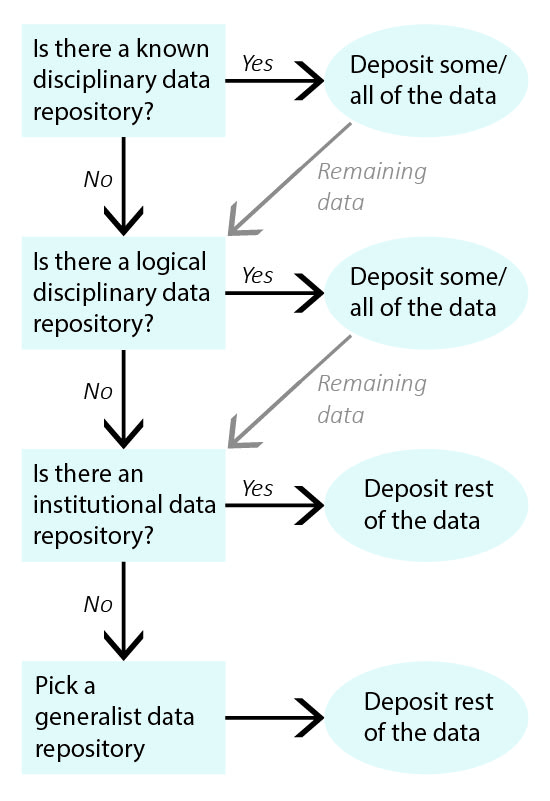
\includegraphics{images/06_Repository.jpg}
\caption{Workflow diagram upon which the exercise is based. Starting at the top, decide is there is a known disciplinary data repository (if so, deposit data), a logical disciplinary data repository (if so, deposit data), an institutional data repository (if so, deposit data), and if none of those work pick a generalist data repository.}
\end{figure}

\begin{center}\rule{0.5\linewidth}{0.5pt}\end{center}

\textbf{1. Identify all of the data that needs to be shared.}

\emph{Example: My data to be shared includes: 1) genetic data for Drosophila; and 2) microscope images of flies.}

~

~

~

\textbf{2. Is there a known disciplinary data repository for some or all of the data? For example, is there a data repository used by everyone in your research area or required for your data type by your funding agency?}

If so, deposit some or all of your data there. Go to step 7 if the repository will accept all of your data or go to the next question if there is still some data left to deposit.

\emph{Example: The database \href{http://flybase.org/}{FlyBase} is used for Drosophila genes and genomes. My genetic data will be shared there.}

~

~

~

\textbf{3. Review the \href{https://journals.plos.org/plosone/s/recommended-repositories}{list of recommended data repositories from PLOS} \citep{plos_one_recommended_2023}. Is there a logical disciplinary data repository for some or all of your data?}

If so, deposit some or all of your data there. Go to step 7 if you have shared all of your data or go to the next question if there is still some data left to deposit.

\emph{Example: There isn't a logical disciplinary data repository for microscope images of flies.}

~

~

~

\textbf{4. Does your institution have a data repository?}

If so, deposit the remainder of your data there and go to step 7.

\emph{Example: The California Institute of Technology hosts the data repository \href{https://data.caltech.edu/}{CaltechDATA}. I will deposit my microscope images in CaltechDATA.}

~

~

~

\textbf{5. Do you have a preferred \href{https://sharing.nih.gov/data-management-and-sharing-policy/sharing-scientific-data/generalist-repositories}{generalist data repository} \citep{nih_generalist_2023}?}

If so, deposit the remainder of your data there and go to step 7.

\emph{Example: {[}All data has been shared already.{]}}

~

~

~

\textbf{6. Pick a \href{https://sharing.nih.gov/data-management-and-sharing-policy/sharing-scientific-data/generalist-repositories}{generalist data repository} \citep{nih_generalist_2023} and deposit the remainder of your data.}

Deposit your data and go to step 7.

\emph{Example: {[}All data has been shared already.{]}}

~

~

~

\textbf{7. Record the permanent identifier, ideally a DOI, from each data deposit.}

DOIs make data FAIR \citep{wilkinson_fair_2016} and aid with data sharing compliance. If you did not receive a permanent identifier (such as a DOI, permanent URL, etc.) during deposit, return to step 2 and pick a different data repository for your data.

\emph{Example: CaltechDATA provides DOIs for all deposits; my permanent identifier is doi.org/10.22002/XXXXXXXXXXX. FlyBase provides stable links to data reports using FlyBase ID numbers; my permanent identifier is flybase.org/reports/FBXXXXXXXXX.}

~

~

~

\hypertarget{share-data}{%
\section{Share Data}\label{share-data}}

\textbf{\emph{Description:}} \emph{Data sharing is becoming common and expected by funding agencies and journals. While the process of depositing data into a data repository will vary between repositories, there are some common actions that should be taken to prepare data for sharing. This exercise walks you through these standard requirements for sharing data.}

\textbf{\emph{Instructions:}} \emph{This checklist enumerates the necessary steps and decisions to deposit data supporting a research article into a data repository. Identify the data to be shared and work through the list. Note that, if data will be shared as multiple deposits or in multiple repositories, the checklist should be worked separately for each group of data.}

\begin{center}\rule{0.5\linewidth}{0.5pt}\end{center}

\textbf{Data Selection}

\_\_ Select the data files that reproduce published results.

\_\_ Perform quality control on the data files.

\_\_ Convert data in proprietary file types to open file types, as appropriate (see \protect\hyperlink{file-type}{Exercise 7.2: Convert Data File Types}).

\_\_ Determine if data should be shared under one citation or as several citations. (Group data as makes most sense for citation and reuse. Options can include: sharing as one large group, grouping files by data type, giving large data files their own citations, etc. Each citation represents a unique deposit into a data repository.)

\_\_ If there will be multiple deposits in one repository or data will be divided across more than one data repository, work through the remainder of the checklist separately for each citation/group of files.

\textbf{Data Documentation}

\_\_ Document any spreadsheet data with a data dictionary (see \protect\hyperlink{data-dictionary}{Exercise 2.3: Create a Data Dictionary}). The data dictionary should be shared with the other files.

\_\_ Write a brief description of each data file, including any data dictionaries, and what it contains. Save this information as a README.txt file and share it with the other files.

\textbf{Sharing Information (Metadata)}

\_\_ Give the dataset a title. Default title is ``Data from: {[}name of the article{]}''.

\_\_ Write a brief description of the dataset to be used as the abstract/description.

\_\_ Write down keywords/subject terms for the data.

\_\_ Determine who will be listed as authors of the data and in what order; this may be different than the authors of the article.

\_\_ Identify author ORCID numbers for submission (note: this is best practice but not all data repositories have integrated ORCID yet).

\_\_ Record all funding information that applies to the dataset.

\_\_ Chose a license for reuse rights. Default license is CC0 (for more information on CC0, see \citep{creative_commons_wiki_cc0_2014}).

\textbf{Deposit Data}

\_\_ Pick a data repository/data repositories for the shared data (see \protect\hyperlink{data-repository}{Exercise 6.1: Pick a Data Repository}).

\_\_ Deposit the data and documentation files into the data repository, and fill in metadata as determined above.

\_\_ If you are depositing a large number of datasets, contact repository administrators about potentially using an Application Programming Interface (API) to skip manual entry of duplicate metadata.

\textbf{Share Data}

\_\_ Share data with its DOI or, as applicable, other permanent identifier.

\_\_ Link the publication to its data, either in a Data Availability Statement or as a citation.

\hypertarget{project-wrap-up}{%
\chapter{Project Wrap Up}\label{project-wrap-up}}

The end of a project is a key time to perform data management activities in order to set yourself up for future data reuse. This is because you still remember all of the important details about your data and can make good decisions about preparing it for the future. This chapter has three exercises to work through for project wrap up: a worksheet on converting data to more open file types; a checklist for populating a project Archive folder; and a checklist for preparing data for reuse, which leverages the previous two exercises.

This chapter also covers project wrap up in the form of separating from your institution. This checklist exercise for the departing researcher is important to work through so that critical data does not get lost in the transition. A fuller version of this checklist, intended for both the departing personnel and a project administrator to work through together, is also available \citep{goben_data_2023}.

\hypertarget{future-use}{%
\section{Prepare Data for Future Use}\label{future-use}}

\textbf{\emph{Description:}} \emph{The end of a project is a good time to prepare data for potential future reuse, as you still know the important details about the data to record and have access to any software used to create the data. This checklist exercise walks you through steps to gather your data into a central place and document the project. Working through the checklist results in project data being in one central location, well documented, and organized and formatted in a way to make future reuse easier.}

\textbf{\emph{Instructions:}} \emph{Gather all of the data from a project and work through the checklist to organize and document the data for future reuse. This exercise refers to several other exercises in the Workbook that should be completed during this process, if they have not been already}

\textbf{\emph{Source:}} \emph{This exercise was adapted from the ``Project Close Out Checklist'' \citep{briney_project_2020}.}

\begin{center}\rule{0.5\linewidth}{0.5pt}\end{center}

\textbf{Prepare Data}

\_\_ Move all data into one central project folder; this folder may have sub-folders and should be organized however makes sense for your data.

\_\_ As necessary, work through \protect\hyperlink{file-type}{Exercise 7.2: Convert Data File Types} to copy data into more open/common file formats.

\textbf{Back Up Your Research Notes}

\_\_ If your notes are electronic, save a copy in the project folder

\_\_ If your notes are physical, scan them and save a copy in the project folder.

\textbf{Create a Project Archive Folder}

\_\_ Work through \protect\hyperlink{archive-folder}{Exercise 7.3: Create an Archive Folder}.

\_\_ Put the Archive folder in the project folder.

\textbf{Create a Project-Level README File}

\_\_ If you haven't done so already, work through \protect\hyperlink{readme-txt}{Exercise 2.2: Project-Level README.txt}.

\_\_ Store a copy of the README file with the data.

\textbf{Save Files in a Stable Location}

\_\_ Save the project folder on a storage system that you will have access to for the next several years.

\hypertarget{file-type}{%
\section{Convert Data File Types}\label{file-type}}

\textbf{\emph{Description:}} \emph{Data is often stored in a file type that can only be opened by specific, costly software -- this is referred to as a ``proprietary file type.'' You can tell that you have data in a proprietary file type if you lose access to the data when you lose access to the software. When data is in a proprietary file type, it's always a good idea to copy the data into a more common, open file type as a backup; you may lose a bit of functionality, but it's better to have a backup than to not have your data at all! This exercise works through identifying possible alternative file types for the data's proprietary file type before instructing you to make a copy of the data in the new file type.}

\textbf{\emph{Instructions:}} \emph{For any data in a proprietary file type, identify the data and answer the following questions. Once you have picked a more open, common file type, make a copy of the data in that file type but do not delete the original data. (Keeping a copy in the original file format means that, while you access to the necessary software, your data has full functionality. If you lose access to the software, you'll still have your data in some format, which is better than not having your data at all.)}

\begin{center}\rule{0.5\linewidth}{0.5pt}\end{center}

\textbf{Is your data stored in a proprietary file type? What file type and how does this limit future data reuse?}

\emph{Example: Data is stored in a .CZI file format, which is a proprietary Zeiss microscope image format. These files do not open in other software.}

~

~

~

\textbf{Is it possible to convert your data to other file types? If so, list the possible types:}

\emph{Example: I can use the Bio-Formats tool to convert .CZI files to: .AVI, .CH5, .DCM/.DICOM, .EPS/.EPSI/.PS, .ICS/.IDS, .JPG, .JP2/.J2K/.JPF, .MOV, .OME.TIFF/.OME.TIF, .OME/.OME.XML, .PNG, or .TIFF/.TIF.}

~

~

~

\textbf{Which of the possible file types are in common use? Which of the possible file types can be opened by multiple software programs?}

\emph{Example: JPG, PNG, and TIFF are all image formats in common use. OME-TIFF is a common image format within microscopy; most software will read the TIFF portion of the file but only some software will read the extra OME metadata. Common movie file types are AVI and MOV.}

~

~

~

\textbf{Of the possible options above, do you have a preference for a specific file type?}

\emph{Example: I prefer an image file over a movie file. TIFF is best because it doesn't lose resolution due to compression and can store all of the 4-dimensional image layers. OME-TIFF gives all of the benefits of TIFF but with added metadata.}

~

~

~

\textbf{Pick one of the more open or common file types and copy your important data files into that file type. Do not delete the original files.}

\emph{Example: I will convert my data to OME-TIFF files.}

~

~

~

\hypertarget{archive-folder}{%
\section{Create an Archive Folder}\label{archive-folder}}

\textbf{\emph{Description:}} \emph{To save your future-self time spent digging through all of your research files, set aside the most important files into a separate ``Archive'' folder. Do this at the end of the project while you still remember which files are important and where they are located. The Archive folder should only contain a small subset of the most important documents that are likely to be reused; you may still need to go through all of your files but, in the majority of instances, you will save time by easily finding what you need in the Archive folder.}

\textbf{\emph{Instructions:}} \emph{This exercise consists of a checklist of the key documents that are likely to be most useful in a research project archive. Create a separate folder within the larger project folder (or in a highly visible place within the storage system) labelled ``Archive''. Copy -- do not move -- the files on this checklist into the Archive folder. Add copies other important research documents, as needed. Remember, the Archive folder does not need to be comprehensive, so focus on the subset of files that are most likely to be reused or referenced in the future.}

\textbf{\emph{Source:}} \emph{This exercise was adapted from the ``Project Close Out Checklist'' \citep{briney_project_2020}.}

\begin{center}\rule{0.5\linewidth}{0.5pt}\end{center}

\textbf{Project Documentation}

\_\_ README file of project information

\textbf{Data Snapshots}

\_\_ Important raw data

\_\_ Key data analyses

\_\_ Final published data

\textbf{Code}

\_\_ Analysis code

\_\_ Record software version, as appropriate

\textbf{Other Research Documents}

\_\_ Protocols

\_\_ Survey instruments

\textbf{Research Notes}

\_\_ Scans of research notebook

\_\_ Digital notes

\textbf{Images}

\_\_ Flat files of figures (e.g.~.JPG or .TIFF)

\_\_ Editable image files (e.g.~.XLSX or .PSD)

\textbf{Publications}

\_\_ Published articles in .PDF format

\_\_ Accepted version of articles in editable document format (e.g.~.DOCX)

\_\_ Poster files

\textbf{Administrative Documents}

\_\_ Grant proposals

\_\_ Grant progress reports and final report

\hypertarget{separation}{%
\section{Separate from the Institution}\label{separation}}

\textbf{\emph{Description:}} \emph{Researchers regularly leave institutions in order to take new jobs. For how common this occurrence is, it represents a critical transition during which data may be lost. This checklist enumerates a number of important steps that researchers can take to ensure that they retain the appropriate data yet leave behind what belongs to the institution.}

\textbf{\emph{Instructions:}} \emph{The researcher leaving the institution should work through this checklist to ensure they keep the proper information while returning what does not belong to them. The researcher and project administrator may also jointly work through the extended version of this exercise, the Data Departure Checklist \citep{goben_data_2023}.}

\textbf{\emph{Source:}} \emph{This exercise was adapted from the ``Data Departure Checklist'' \citep{goben_data_2023}.}

\begin{center}\rule{0.5\linewidth}{0.5pt}\end{center}

\textbf{Retain Copies of Data that You Have Permission to Keep}

\_\_ If you have not done so already, work through \protect\hyperlink{data-governance}{Exercise 5.2: Determine Data Stewardship} to determine what data you may retain

\_\_ Identify and keep pertinent research data from personal devices

\_\_ Identify and keep pertinent research data from storage systems (e.g.~AWS/Azure, Box, campus HPC, Dropbox, Electronic Lab Notebook, Globus, Google Drive, lab/department/college servers, Microsoft OneDrive, Microsoft Sharepoint, or shared collaborator drives)

\_\_ When appropriate, make a copy of research notes

\textbf{Delete Personal Information and Remove Personal Devices}

\_\_ Remove personal information from lab devices

\_\_ Remove personal devices from lab

\_\_ Remove personal access to shared accounts (e.g.~lab Github, lab repository page, lab website, mailing lists, or social media)

\textbf{Return Lab Hardware}

\_\_ Individual computer / workstation

\_\_ Tablet(s)

\_\_ Peripherals (e.g.~keyboard, mouse, monitor)

\_\_ External drives

\_\_ Other lab equipment (e.g.~cameras, recording devices)

\textbf{Update Research Administration Documents, As Necessary}

\_\_ Update/transfer Institutional Review Board

\_\_ Update/transfer IACUC

\_\_ Update/transfer Data Use Agreements (DUA)

\_\_ Update/transfer Material Transfer Agreements (MTA)

\_\_ Update/transfer research grants

\textbf{Handle Email}

\_\_ Set out of office, providing forwarding information

\_\_ Forward/backup important emails

\_\_ Check with University Archivist or Records Manager for retention policies (depends on rank)

\hypertarget{acknowledgements}{%
\chapter*{Acknowledgements}\label{acknowledgements}}
\addcontentsline{toc}{chapter}{Acknowledgements}

This book came to me at a moment when I was looking for a new big project. I was washing my hands and BAM! the idea for this book erupted in my head, fully formed like Athena from the head of Zeus. Prior to writing the Workbook, I had created several data management handouts and worksheets to use in lectures and workshops. My big idea was to expand my worksheet offerings to cover the entire data management lifecycle. Basically, I wanted a workbook of activities to pull from for any data management lesson I taught. The result is this Workbook.

Books are never truly written by only one person. While I did the majority of the labor for this Workbook, it would not have been as helpful, accurate, or complete without the assistance of several people.

First, thank you to several people at Caltech Library for assistance with this book. Thank you Donna Wrublewski for being on board with this big idea and supporting it. Big thanks to Tom Morrell for critical feedback on the beta edition of this book, particularly on the storage exercise which was really terrible before his feedback. Thank you Tommy Keswick for helping move my bookdown repo to the Caltech Library GitHub account and for showing me the magic that is GitHub Pages. Thank you to George Porter for helping to get the Workbook online into CaltechAUTHORS, even though we were not quite finished migrating that giant repository to its new platform.

Thank you to Abigail Goben and Dorothea Salo for always being encouraging when I come to them with the idea for a new book, no matter the idea. Abigail was one of the first people I discussed the idea for this book with, which helped cement the big idea in my head. Dorothea read and provided feedback and editing, which was greatly appreciated.

Finally, thank you to Andy for being calm when I had the idea for yet another book. It helped that this book was much shorter than my last two. And thank you to Hank and Willa for cuddles, questions, and all of our adventures that keep me grounded.

  \bibliography{references.bib}

\end{document}
